% ****** Start of file apssamp.tex ******
%
%   This file is part of the APS files in the REVTeX 4.1 distribution.
%   Version 4.1r of REVTeX, August 2010
%
%   Copyright (c) 2009, 2010 The American Physical Society.
%
%   See the REVTeX 4 README file for restrictions and more information.
%
% TeX'ing this file requires that you have AMS-LaTeX 2.0 installed
% as well as the rest of the prerequisites for REVTeX 4.1
%
% See the REVTeX 4 README file
% It also requires running BibTeX. The commands are as follows:
%
%  1)  latex apssamp.tex
%  2)  bibtex apssamp
%  3)  latex apssamp.tex
%  4)  latex apssamp.tex
%
\documentclass[%
 reprint,
%superscriptaddress,
%groupedaddress,
%unsortedaddress,
%runinaddress,
%frontmatterverbose,
%preprint,
%showpacs,preprintnumbers,
%nofootinbib,
%nobibnotes,
%bibnotes,
 amsmath,amssymb,
 aps,
 norsk,
 booktabs
%pra,
%prb,
%rmp,
%prstab,
%prstper,
%floatfix,
]{revtex4-1}

\usepackage[utf8]{inputenc}
\usepackage[norsk]{babel}
\usepackage{varioref}
\usepackage{graphicx}% Include figure files
\usepackage{enumitem}
\usepackage{dcolumn}% Align table columns on decimal point
\usepackage{bm}% bold math
\usepackage[margin=0.9in]{geometry}
\usepackage[mathlines]{lineno}% Enable numbering of text and display math
%\linenumbers\relax % Commence numbering lines

\usepackage[usenames,dvipsnames,svgnames,table]{xcolor}
\usepackage[colorlinks]{hyperref}
\usepackage{relsize}
%\usepackage{booktabs}
\usepackage{graphicx,verbatim,amsfonts,geometry}
\usepackage{amsmath}
\newcommand*\diff{\mathop{}\!\mathrm{d}}
\newcommand*\Diff[1]{\mathop{}\!\mathrm{d^#1}}
\usepackage{ulem}
\usepackage{amssymb}
\usepackage{multirow}
\usepackage{soul}
\usepackage{dsfont}
% allows for temporary adjustment of side margins
\usepackage{chngpage}
% just makes the table prettier (see \toprule, \bottomrule, etc. commands below)
\usepackage{booktabs}

\usepackage{commath}
\usepackage{wrapfig}
\usepackage[free-standing-units=true]{siunitx}
\DeclareSIUnit\year{yr}
\usepackage{gensymb}
\newcommand{\ROM}[1]{%
  \textup{\uppercase\expandafter{\romannumeral#1}}%
}
\usepackage{physics}
\usepackage{caption}
\usepackage{bm}
\usepackage{gensymb}

\makeatletter
\newcounter{elimination@steps}
\newcolumntype{R}[1]{>{\raggedleft\arraybackslash$}p{#1}<{$}}
\def\elimination@num@rights{}
\def\elimination@num@variables{}
\def\elimination@col@width{}
\newenvironment{elimination}[4][0]
{
    \setcounter{elimination@steps}{0}
    \def\elimination@num@rights{#1}
    \def\elimination@num@variables{#2}
    \def\elimination@col@width{#3}
    \renewcommand{\arraystretch}{#4}
    \start@align\@ne\st@rredtrue\m@ne
}
{
    \endalign
    \ignorespacesafterend
}
\newcommand{\eliminationstep}[2]
{
    \ifnum\value{elimination@steps}>0\sim\quad\fi
    \left[
        \ifnum\elimination@num@rights>0
            \begin{array}
            {@{}*{\elimination@num@variables}{R{\elimination@col@width}}
            |@{}*{\elimination@num@rights}{R{\elimination@col@width}}}
        \else
            \begin{array}
            {@{}*{\elimination@num@variables}{R{\elimination@col@width}}}
        \fi
            #1
        \end{array}
    \right]
    &
    \begin{array}{l}
        #2
    \end{array}
    \addtocounter{elimination@steps}{1}
}
\makeatother
% Document formatting
\setlength{\parindent}{0mm}
\setlength{\parskip}{1.5mm}

\begin{document}

\title{Solcelle}
\author{\textsc{Ivar Svalheim Haugerud}}
\affiliation{ Universitetet i Oslo}
\date{\today}

\begin{abstract}
Eksperimentelle målinger på strømmen gjennom og spenningen over en solcelle ble gjennomført under forskjellige koblinger og belysninger, for å forstå forholdet mellom kobling og belysning, og maksimal effekt. Den maksimale effekten til en solcelle er en viktig egenskap for å få mest ut av solcellepaneler. Solcellene brukt i dette eksperimentet har vært i krets alene, i serie og i parllell, under varierte lysforhold. Målingen av strøm-spenningkarakteristikken til solcellen, i positiv og negativ lederretning, viser at solceller er dioder. Fra å analysere støm-spenningkarakteristikken og bruke dette til å beregne maksimale effekt viser det seg at den optimale resistansbelastningen til en solcelle avhenger av belysningen til solcellen. Dette blir analysert videre ved å koble solceller i serie og parallell. Å koble solceller i parallell øker strømmen, å koble solceller i serie øker spenningen i kretsen, effekten vil være tilnærmet den samme for de to koblingsmåten. Derimot hvis en belyser en solcelle, istedenfor to, måler man en faktor $263(3)$ mer maksimal effekt fra å ha solcellene koblet i parallel istedenfor i serie. Parallellkoblede solceller gir en faktor $2.04(1)$ mer effekt av at begge solcellene er belyst, for seriekoblede øker effekten med $512(7)$ av at begge solcelle belyst iforhold til en. Ved å bruke et solarimeter ble det målt at virkningsgrad til solcellen brukt i dette eksperimentet er på $7.35(3)\%$.
\end{abstract}

\pacs{Valid PACS appear here}% PACS, the Physics and Astronomy
                             % Classification Scheme.
%\keywords{Suggested keywords}%Use showkeys class option if keyword
                              %display desired
\maketitle

%\tableofcontents
\section{Introduksjon}
Eksperimentet i denne rapport ble gjennomført i håp om å forstå hvordan å maksimere effekten til en solcelle, og hvilken virkningsgrad en solcelle har. En god solcelle skal genere mest mulig elektrisk energi under forskjellige belysninger og koblinger. Vi skal derfor gjør målinger i elektriske kretser som inneholder belyste solceller for å finne den maksimale effekten solcellen klarer å genere, og studere hvordan denne maksimale effekten varierer under forskjellige koblingsmåter og belysninger.\\
Solceller omdanner lys til elektrisk strøm. Dette kan gjøres ved hjelp av halvlederteknologi. For solceller er det vanlig å bruke en halvleder laget av silisiummateriale. Halvledermaterialet gjør at negative ladninger, elektroner, lagrer seg i den ene halvlederen, mens positive ladninger, elektronhull, på den andre. Når et foton treffer overgangsområdet mellom de to halvlederene vil det bli dannet et elektron-hull-par. På grunn av ladningsforskjellen mellom de to halvlederene vil elektronet og hullet bevege seg i hver sin retning, som danner en strøm. For å kunne utnytte utnytte strømmen er det koblet metallkontakter som forbinder de to halvlederene. I denne metallkontakten vil det dannes en strøm som kan utnyttes \cite{snl}.\\
Eksperimentet som skal gjennomføres består av fire hoveddeler. Vi skal se på solcellen som en halvlederdiode (1) ved å måle strøm-spenningskarakteristikken til solcellen. Dette skal måles med og uten en ytre spenningskilde. For å teste diode-egenskapen til solceller skal målingene bli gjort i lederretning, og i sperreretning. Disse målingene kan brukes videre til å måle solcellens optimale belastning (2). Disse målingene skal gjøres med solcellen direkte belyst, og delvis belyst, for å finne forholdet mellom maksimal effekt i de to tilfellene. Maksimal effekt skal studeres litt nærmere ved å gjøre målinger på hvordan kombinasjon av enkeltsolceller i et solcellepanel påvirker maksimal effekt (3). Dette blir gjort ved å finne maksimal effekt under forskjellige belysninger for serie og parallellkobling av to solceller. Til slutt blir det gjennomført målinger for å finne hvor mye av den innkommende lys-energien som blir omgjort til elektrisk energi, ved å finne solcellens virkningsgrad (4). Fra de fire forskjellige målingene ønsker vi å få en bedre forståelser til virkemåten til solceller, og finne hvordan koblingsmåte og belysning påvirker maksimal effekt. \\
Hensikten med gode solceller er lett å se nytten av. Som det blir et økende antall mennesker på jorden, og man starter å innse de ødeleggende konsekvensene av et stort forbruk av olje og gass, har det blitt en stor vekst innenfor fornybare energikilder, spesielt vindkraft og solceller \cite{oppgave}. Solceller har en stor, og tilnærmet evigvarende energikilde å tappe energi fra, solen. Hvert sekund blir hver kvadratmeter av jordoverflaten bestrålt av solenergi på $\SI{1370}{\joule}$ \cite{snl2}. Deler av energien blir absorbert i skyer og støv, men gjennomsnittlig vil jordoverflaten på ekvator midt på en klar dag absorbere energi på rundt $\SI{950}{\joule}$ per kvadratmer hvert sekund \cite{oppgave}. Iløpet av et år tilsvarer dette rundt $15 000$ ganger jordens årlig energiforbruk \cite{snl2}. Selv om vi klarer å utnytte energi fra solen, er man ikke fornøyd med andel av energien man klarer å utnytte. Komersielle solceller klarer å utnytte mellom $15-22\%$ av energien som treffer jordoverflaten \cite{oppgave}. Forskning innenfor solceller prøver å gjøre det rimeligere å produsere, og øke andelen av energien en får utnyttet. Vi ønsker derfor i dette eksperimentet å studere hvordan å maksimere effekten generert fra en solcelle under forskjellige belysninger.
\section{Teori}
\subsection{Kretsteori}
I starten av det forrige århundet oppdaget man uttrykket for energien til et foton. Dette uttryket viser at energien $E$ til et foton er propsjonal med frekvensen, $\nu$, til fotonet
\begin{equation}
  E = h\nu = \frac{hc}{\lambda} \label{einstein},
\end{equation}hvor $h$ er Plancks konstant, $c$ er lyshastigheten, og $\lambda$ er bølgelengden til fotonet. Denne relasjonen ble påvist av Einstein i 1905 ved å forklare den fotoelektriske effekt. Akkurat som den fotoelektriske effekt kommer solcellen i dette eksperimentet til å være koblet i en krets med forskjellige komponenter. Den viktigste relasjonen vi kommer til å bruke er Ohms lov
\begin{equation}
  V = RI,
\end{equation}som sier at spenningsfallet $V$ over en komponent er gitt av produktet mellom strømmen $I$ og resistansen $R$ til komponenten. Dette kan brukes for å finne effekttapet, $P$, til en komponent, som er gitt av produktet mellom spenningsfallet over komponenten og strømmen som går gjennom den
\begin{equation}
  P = VI = RI^2 = \frac{V^2}{R} \label{effekt1}.
\end{equation}For å få lage den beste mulige solcellen burde effekten $P$ være så stor som mulig. Vi kommer derfor til å trenge noen viktige relasjoner for den maksimale effektiviteten $P_{max}$. Under eksperimentet kommer vi til å gjøre målinger for å finne strøm-spenningskarkateristikken til solcellen. Vi kommer derfor til å finne solcellens spenning med uendelig stor motstand, det vil si \textit{open circuit}, $V_{oc}$. Dette er den maksimale spenningen solcellen kan danne. Og det motsatte, hvilken strøm som går i solcellen når det er tilnærmet ingen motstand i kretsen, den er kortsluttet, det vil si \textit{short circuit}, $I_{sc}$. Dette er den maksimale strømmen solcellen klarer å generere. Det viser seg at forholdet mellom den maksimale effekten og produktet av $V_{oc}$ og $I_{sc}$ er konstant, og har fått navnet \textit{fill factor}.
\begin{equation}
  \frac{P_{max}}{V_{oc}I_{sc}} = FF. \label{ff}
\end{equation}
Som den maksimale effekten kan sees på som det maksimale arealet i strøm-spenningkarakterstikken, er produktet av $V_{oc}$ og $I_{sc}$ arealet til utspent av skjæringspunktene i strøm-spenningkarakterstikken. Det denne likningen sier er at forholdet mellom disse to arealene er tilnærmet proposjonalt for samme solcelle. Og denne proposjonalitetskonstanten kalles \textit{fill factor}. Verdien til fill factor forteller hvor mye effekt solcellen klarer å produsere. Vanligvis er verdien på rundt $0.7$ til $0.8$, jo nærmere forholdet er $1$, jo mer effekt får man fra kretsen.\\
Relasjonen i likning \eqref{ff} er en nyttig relasjon når vi skal studere forholdet mellom effekter. Årsaken til dette er et fill factor er en karakteristikk av solcellen, og er ikke avhengig av eksterne forhold. Siden fill factor er tilnærmet lik konstant kan vi finne forholdet mellom to effekter for samme solcelle i forskjellige situasjon, ved å bruke definisjonen av fill factor
\begin{equation}
  \frac{\left(P_{max}\right)_1}{\left(P_{max}\right)_2} \approx \frac{\left(V_{oc}I_{sc}\right)_1}{\left(V_{oc}I_{sc}\right)_2}. \label{maxP}
\end{equation}Hvor måling $1$ og måling $2$ kan henvise til f.eks målinger av samme solcelle, men med forskjellig belysning eller forskjellig kobling.\\
For å beregne virkningsgraden til solcellen blir det brukt et solarimeter under eksperimentet. Solarimeteret har en kalibreringskonstant $a$ som gjør det mulig å beregne den bestrålte effekten på solcellen. Den bestrålte effekten er gitt av produktet mellom spenningen over solarimeteret $V_s$ og arealet $A$ til solcellen, som må divideres på kalibreringskonstanten $a$
\begin{equation}
  P_{inn} = \frac{V_sA}{a} \label{kalibrering}.
\end{equation}
Ved å vite $P_{inn}$ kan en beregne virkningsgraden ved å sammenlikne denne verdien med den maksimale effekten målt fra solcellen $P_{max}$. Dette gjøres ved
\begin{equation}
  \text{effekt} = \frac{P_{max}}{P_{inn}}\cdot 100\%\label{effekt}.
\end{equation}
%I eksperimentet skal det gjennomføres målinger av strøm-spenningkarakteristikken til en solcelle. Dette skal gjøres med og uten en ytre kilde, både i positiv og negativ lederretning.
\subsection{Halvledere og solceller}
De fleste solceller er laget av halvledermateriale, for å forstå solceller må en derfor forstå halvledere. Halvledere fungerer på grunn av kvanatiserte energinivåer til atomer. Elektroner i atomer oppbevarer seg på elektronskall som tilsvarer kvantetallet deres, $n\in\mathbb{N}$. For hvert energinivå er det oppdelt i underskall som blir bestemt av det azimutale kvantetallet $l \in \mathbb{N} < n$. Denne elektronkonfigurasjonen er forskjellig for forskjellig atomer, og bestemmer de kjemiske og fysiske prosessene til atomet.\\
Bindinger mellom atomer bestemmes av elektronene i de ytterste skallene, dette er elektronene med størst $n$ og derfor høyest energi, som kalles valenselektronene. Ved å tilføre elektroner energi vil elektronene eksiteres, de øker avstanden til kjernen og flytter seg til et høyere skall. Siden energinivåene er kvantiserte vil forflytningen være kvantisert. For like atomer er disse energinivåene identiske, men når vi har flere identiske atomer sammen oppstår det nye effekter, \textit{more is different}. De originiale energinivåene splittes opp til flere forskjellige energinivåer. Antall forskjellige energinivåer øker med antall atomer, og er det nok atomer tilstede vil det bli dannet et kontinuerlig energibånd. Energibåndet som dannes av valenselektroner kalles valensbåndet. Er valensbåndet fullt av elektroner kan ikke elektronene drifte for å danne strøm i valensbåndet. Det blir først mulig å danne strøm hvis elektronene blir eksitert til det neste ikke-okkuperte energibåndet, som er over valensbåndet, dette båndet kalles ledningsbåndet. For silisium, som vi bruker i dette eksperimentet, og andre halvledere, er det et energiområde mellom valensbåndet og ledningsbåndet hvor elektronet ikke kan ha en energitilstand. Dette området kalles båndgapet, for silisium er størrelsen på båndgapet $\SI{1.12}{\electronvolt}$.\par
Halvledere kan beholde krystallstrukturen sin, og forbedre sin elektriske ledningsevne, ved å bli dopet av fremmedatomet. Doping innebærer at man erstatter en svært liten andel ($1/10^6$) av silisiumatomene med andre atomer. For at et fremmedatom skal binde seg til silisiumsgitteret trenger det fire valenselektroner. Arsen har fem valenselektroner, som gjør at det siste valenselektronet blir svakt bundet til arsen-atomet. Dette gjør at det lett kan binde seg til nabo silisium-atomet. Elektronet vil derfor fortsette å kunne bevege seg fra atom til atom inne i krystallen. Siden vi har økt antall elektroner kalles dette $n$-doping, $n$ for negativ. Ved å dope silisium med bor-atomer, som har tre valenselektroner, vil det danne en vandrene hull-strøm. Siden vi har redusert antall elektroner kalles dette $p$-doping, $p$ for positiv.\\
Grensesjiktet mellom to halvledere, der den ene havlederen er $n$-dopet og den andre er $p$-dopet, kalles for en $pn$-overgang. I dette området, \textit{overgangssonen}, vil noen av de fri elektronene fra den $n$-dopede halvlederen fylle hullene i den $p$-dopede halvlederen. Denne forflyningen av ladning fører til ladde ioner på hver side av overgangssonen. Dette gjør at $p$-siden blir netto negativt ladd, og $n$-siden blir netto positivt ladd. Denne ladningsforskjellen mellom de to områdene vil dannet et elektrisk felt fra $n$-området til $p$-området. Dette feltet vil hindre flere elektroner fra å bevege seg over overgangssonen.\\
Vi har beskrevet hvordan halvledere virker, men ikke hvordan dette er relatert til solceller og lys. For å  forstå dette må vi se nøyere på overgangssonen til silisiumatomer. Får ett elektronen tilført energi, ved å absorbere et foton, kan det løsnes fra kjernen og bevege seg fritt i krystallen. Mest sansnylig vil elektronet binne seg med det atomet det ble løsrevet fra, og vi er like langt. Er elektronet i overgangssonen vil retningen på det elektriske feltet gjøre at elektronene blir dratt over til $n$-området, og hullet i retning $p$-området. Spenningsforskjellen har separert elektronet fra hullet. Nå er det et atom på $p$-siden av overgangssonen som har mistet et elektron. Dette hullet kommer til å bli fylt av et annet elektron. Som tiden går vil $p$-området få et overskudd av hull, og $n$-området et overskudd av elektroner. Dette endrer på spenningsforskjell mellom områdene. Nå øker ladningen antall positive ladninger på $p$-siden, og på $n$-siden øker antall negative ladninger. Dette gjør at den tidligere spenningsforskjellen avtar, helt til det ikke er noen ladningsforskjell på de to områdene. Dette fører til at det slutter å være transport av elektroner og hull i overgangssonen. Har nå solcellen blitt ubrukelig? Nei, ved å koble $p$-området med $n$-området ved hjelp av en ytre ledning vil elektroner fra $n$-området strømme til hullene i $p$-området. Kobler man en motstand på ledningen vil det dannes en effekt, som vi skal måle i dette eksperiment. Strømmen av ladninger i ledningen gjør at feltstyrken opprettholdes, og prosessen fortsetter. Strømmen vil fortsette å gå, så lenge lys treffer solcellen.\par
Ikke alt lys vil klare å løsrive elektroner fra atomet. For silisium er energien som trengs $\SI{1.12}{\electronvolt}$. Ved å bruke relasjonen mellom energi og bølgelengde\eqref{einstein} finner vi at det kreves en bølgelengde mindre enn $\SI{1100}{\nano\meter}$ for å løsrive et elektron for å danne et elektron-hull par. Derfor vil alt lys med bølgelengde lengere enn $\SI{1100}{\nano\meter}$ ikke føre til noe strøm i solcellen. Spenningen i solcelle kretsen vil aldri kunne bli større enn energien som kreves å løserive et elektron, per elektron, $V<E/e$. For silisium vil dette bety at spenningen solcellen lager vil alltid være mindre enn $\SI{1.12}{\volt}$. En så lav spenning ville ikke klart å lade opp de fleste batterier for pratktisk nytte. Det er derfor ønskelig å endre på kretsen slik at det kan enten bli høyere spenning, eller høyere strøm i kretsen. For å få høyere spenning kan man koble flere enkeltsolceller i serie, ønskes det høyere strøm kobles det flere enkeltsolceller i parallell. Dette skal vi se nærmere på under eksperimentet.
\section{Eksperimentelt}
Under hele eksperimentet kommer vi til å ha en solcelle i en fast avstand fra en lyskilde. Solcellen plasseren i et stativ på en optisk benk sammen med en lysbildeprosjektor. Avstanden mellom den lyskilden og solcellen er valgt slik at solcellene vi kommer til å bruke under eksperimentet kommer til å være fullstendig belyst. Eksperimentet foregår i ett mørkt rom for å kontrollere belysningen av solcellen.\\
\subsection{Strøm-spenningskarkateristikk}
Vi ønsker å måle strøm-spenningkarakteristikken for en belyst solcelle. Først skal vi finne karakteristikken med en ytre spenningskilde i kretsen, og senere uten en spenningskilde i kretsen.
\subsubsection{Med ytre spenningskilde}
For å finne strøm-spenningkarakteristikken med en ytre spenningskilde blir solcellen koblet i en krets sammen en varierende motstand, en spenningskilde på $5$ volt og to voltmetere. Kretsen er vist i figur \vref{krets1}. For å finne strøm-spenningkarakteristikken må vi måle spenningsfallet over solcellen, og strømmen som går gjennom solcellen. Spenningsfallet over solcellen blir målt av voltmeteret $V$ i figur \vref{krets1}, og strømmen i kretsen blir beregnet fra spenningsfallet over resistansen $R_L$, som vi leser av voltmeteret $V_L$. Under målingene varierer vi størrelsen på motstanden i kretsen, og gjør flere målinger for hver verdi av resistansen, for å begrense usikkerheten i målingene. Vi forventer et knekkpunkt i forholdet mellom strøm og spenning, og vi velger derfor verdier av resistansen slik at vi får mange målinger rundt knekkpunktet. Siden vi ønsker å måle strøm-spenningkarakteristikken både i lederretning (hullstrøm), og i sperreretning (negativ strøm), snur vi polariteten på spenningskilden når vi er fornøyd med målingene i lederretning, og gjentar prosessen.
\begin{figure}[h!]
  \centering
  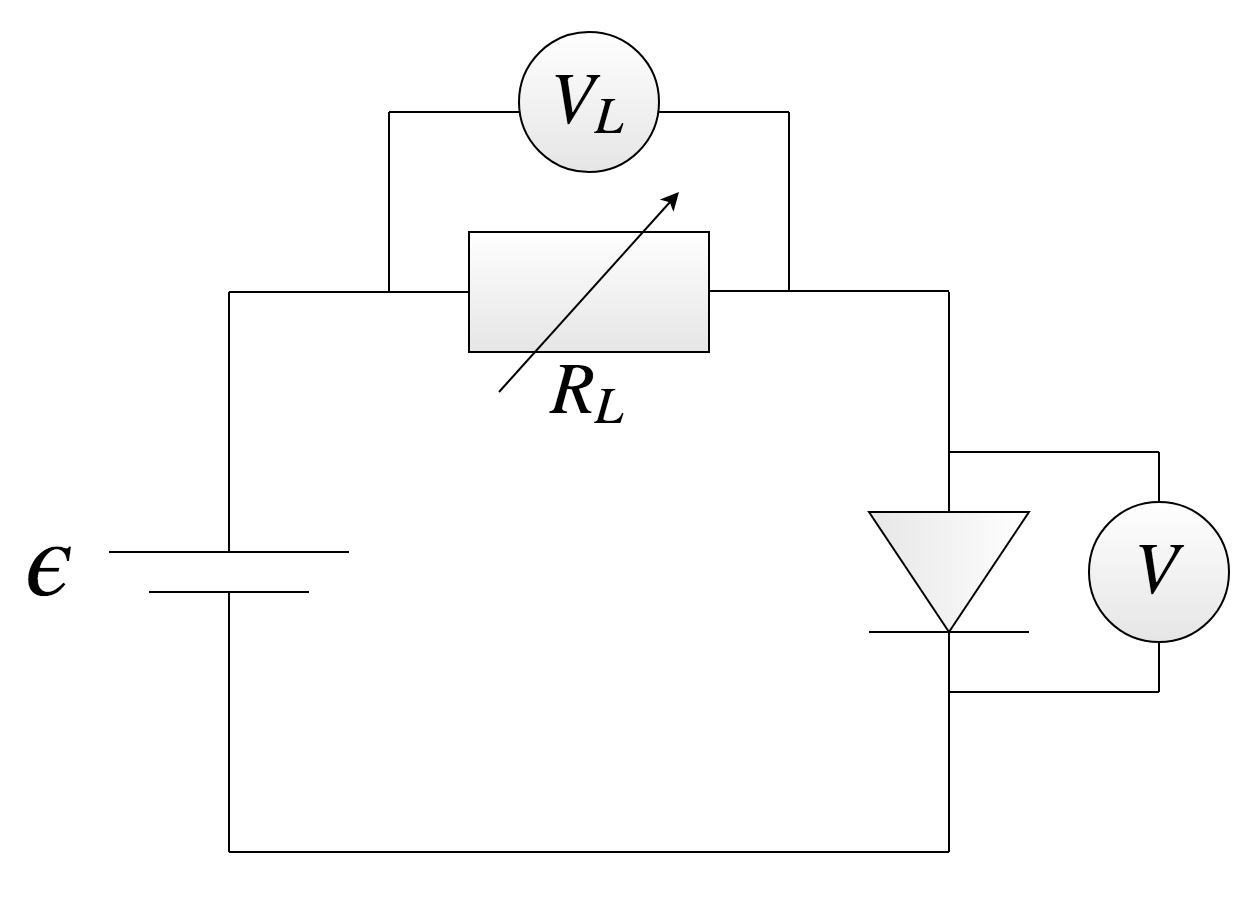
\includegraphics[scale=0.15]{krets1.png}
  \caption{Krets for å måle strøm-spenning karakteristikken til solcellen, med en ytre påtrykket spenning $\epsilon$.}
  \label{krets1}
\end{figure}
\subsubsection{Uten ytre spenningskilde}
Vi ønsker nå å måle strøm-spenningskarkateristikken uten en ytre spenningskilde. Nå skal den eneste spenningskilden i kretsen være solcellen selv. For denne målingen bruker vi kretsen vist i figur \vref{krets2}. Vi skal igjen variere reistansen i motstanden $R_L$ mens vi måler strømmen gjennom, og spenningen over, solcellen. Siden vi også her forventer et knekkpunkt i strøm-spenningkarakteristikken velger vi verdier av motstanden slik at vi får flest målinger rundt dette knekkpunktet. Vi ønsker også å gjøre målinger for å finne spenningen når motstanden $R_L$ går mot uendelig $V_{oc}$. For å gjøre motstanden uendelig stor kobler vi motstanden ut av kretsen, slik at det umulig kan gå strøm gjennom. Verdien for strømmen som går gjennom kretsen når motstanden $R_L$ er null, det vil si $I_{sc}$ strømmen gjennom en åpen krets, finner vi ved å gjøre målinger mens vi lar $R_L$ gå mot null, men aldri bli nøyaktig lik null. Årsaken til at vi ikke kan sette $R_L$ lik null er at da mister vi muligheten til å beregne strømmen $I_{sc}$ i kretsen. Motstanden $R_L$ må være stor nok til at vi kan måle spenningen $V_L$ med en rimelig nøyaktighet.
\begin{figure}[h!]
  \centering
  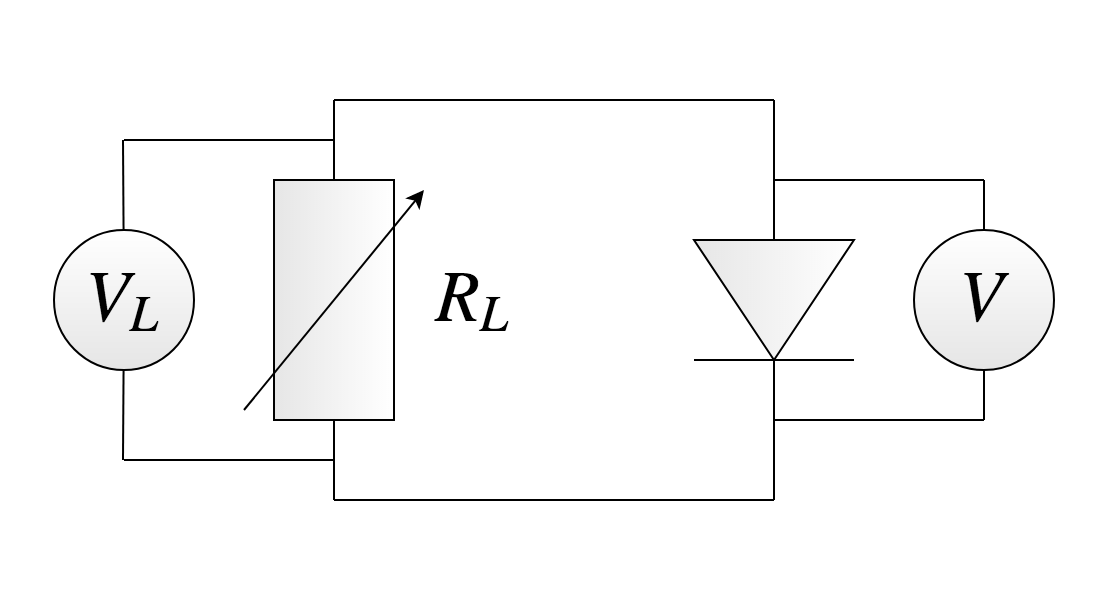
\includegraphics[scale=0.17]{krets2.png}
  \caption{Krets for å måle strøm-spenning karakteristikken til solcellen, uten en ytre påtrykket spenning.}
  \label{krets2}
\end{figure}
\subsection{Solcellens optimale belastning}
Den optimale belastningen på en solcelle vil gi mest mulig effekt fra en belyst solcelle. Effekten beregnes fra å bruke likning \eqref{effekt1}. Det må derfor gjøres målinger av spenningen over motstanden, og strømmen gjennom den. Siden det bare er en komponent i kretsen, utenom solcellen, vil alt spenningsfallet skje over denne komponenten. Dette gjør at vi kan få all informasjonen vi trenger fra å måle spenningsfallet over motstanden, og vite resistansen. Derfor trenger vi nå bare ett voltmeter i kretsen, kretsen som ble brukt er vist i figur \vref{krets3}. Målingene for å finne optimal belastning blir gjort for samme solcelle, men med to forskjellige belysninger. Den ene belysningen er at solcellen er rettet direkte mot lyskilden for å få mest mulig bestråling. Den andre belysningen er at vi roterer solcellen rundt $\SI{60}{\degree}$ slik at strømmen i kretsen, med en lav verdi for $R_L$, er halvert.
\begin{figure}[h!]
  \centering
  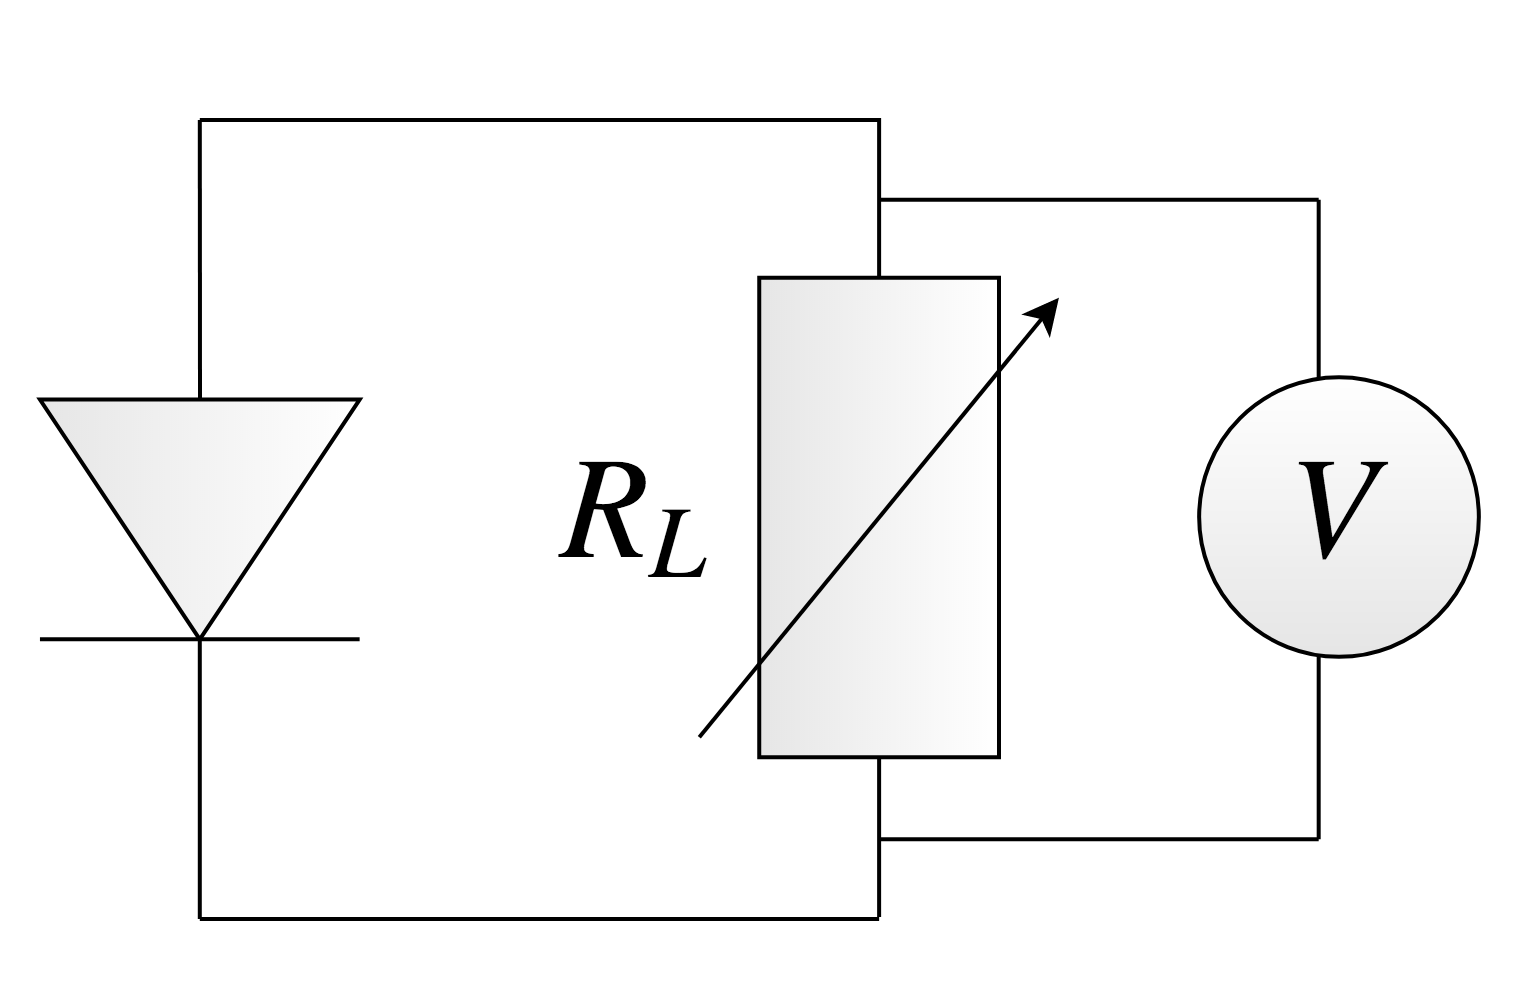
\includegraphics[scale=0.1]{krets3.png}
  \caption{Krets for å måle strøm gjennom og spenning over solcellen, for å finne den optimale belastningen til solcellen.}
  \label{krets3}
\end{figure}
\subsection{Kombinasjon av enkeltsolceller i et solcellepanel}
For å få høyere spenning fra en solcelle kobler man flere i serie, ønsker man høyere strøm kobler man dem i parallell. For å gjøre målinger på denne effekten bruker vi nå to solceller som settes i lik avstand til lyskilden. Det er to forskjellige kretser som blir brukt under målingene. En med sollcellene i parallell, og en med solcellene i serie, disse to er vist i figur \vref{krets4}. For å finne forholdet mellom den maksimale effekten for forskjellige tilfeller bruker vi likning \eqref{maxP}. Dette gjør at de to eneste egenskapene vi trenger å måle er spenningsfallet over resistansen i en åpen krets ($V_{oc}$), og strømmen i en kortsluttet krets ($I_{sc}$).
\begin{figure}[h!]
  \centering
  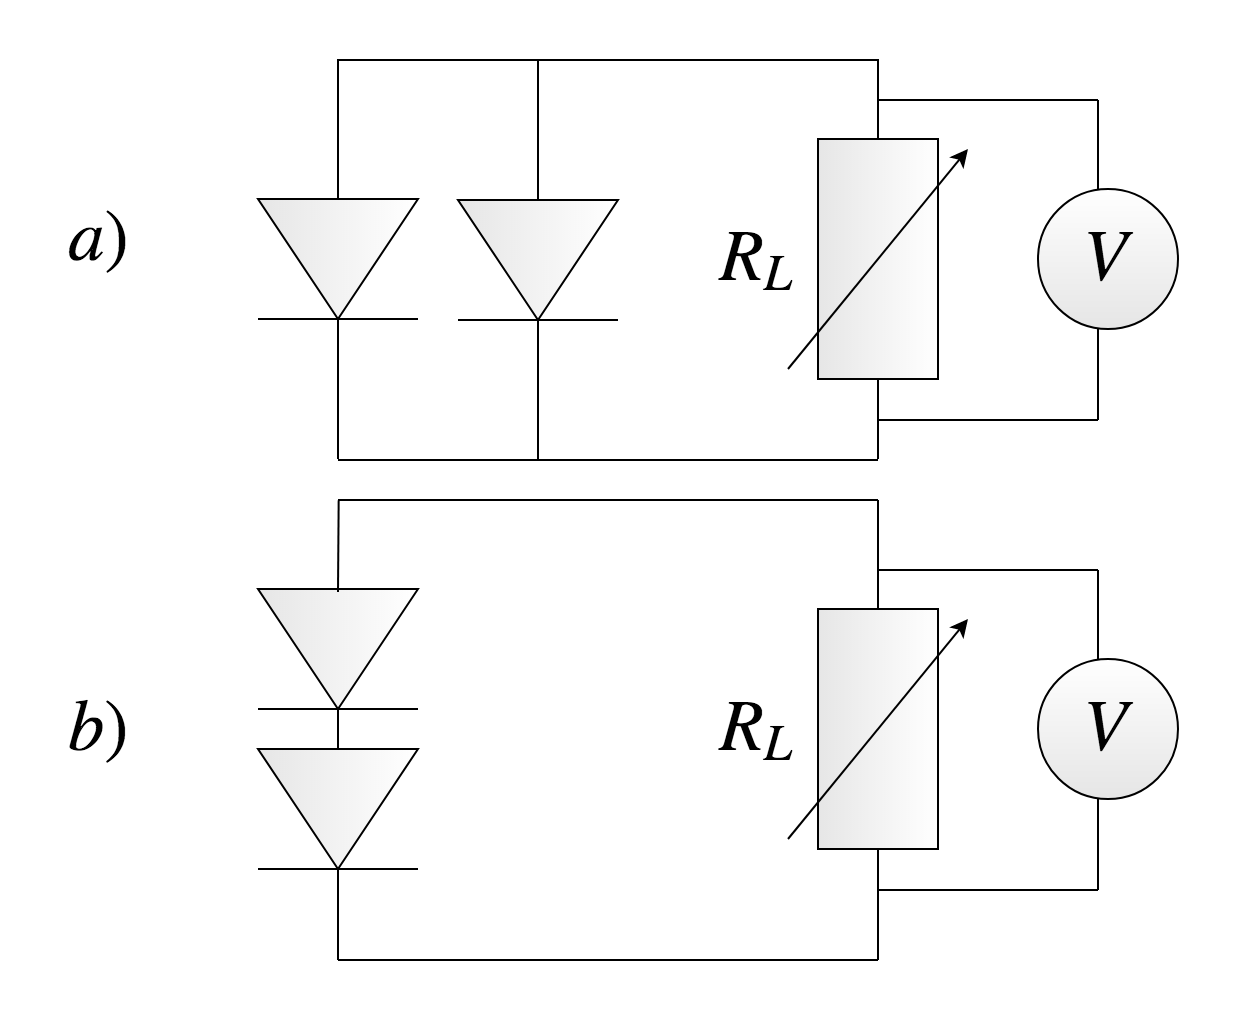
\includegraphics[scale=0.16]{krets4.png}
  \caption{Krets for å måle forskjellen i strøm og spenning når to solceller er koblet i parallell (a) iforhold til i serie (b).}
  \label{krets4}
\end{figure}
For både parallellkoblede solceller og seriekoblede solceller blir det gjort målinger av $V_{oc}$ og $I_{sc}$ for to forskjellige tilfeller. Det første tilfellet er at begge solcellene er belyst like mye. Deretter dekker vi til den ene solcellen og gjør igjen de samme målingene. Fra disse målingene kan man beregne effektivitetsforholdet mellom de to tilfellene med likning \eqref{maxP} for både serie og parallell koblede solceller.
\subsection{Solcellens virkningsgrad}
For å finne virkningsgraden til solcellen må irradiansen måles, det vil si den innfallende strålingseffekten per areal, og finne forholdet mellom denne og andelen som blir omdannet til elektrisk energi. For å måle den innkommende energien blir det brukt et solarimeter. Oppsettet under målingen av solarimeteret er vist i figur \vref{lab1}. Solarimeteret blir plassert ved samme avstand til lyskilden som solcellen, slik at strøm-spenning karakteristikken målt tidligere kan brukes. Det er to mål som må gjøres for å beregne effektiviteten til solcellen. En må måle spenningen over solarimeteret med et følsomt voltmeter, og notere seg kalibreringskonstanten til solarimeteret. Det andre en må målet er arealet til solcellen. Dette blir gjort ved å bruke et skyvelær. Grunnet formen til solcellen var det mange lengder som måtte måles. Spenningen over solarimeteret og arealet av solcellen kan brukes i likning \eqref{kalibrering} for å beregne effekten som solcellen blir belyst. Fra forholdet mellom effekten den blir belyst, og den maksimale effekten i kretsen kan vi beregne effektiviteten til solcellen med likning \eqref{effekt}.
\begin{figure}[h!]
  \centering
  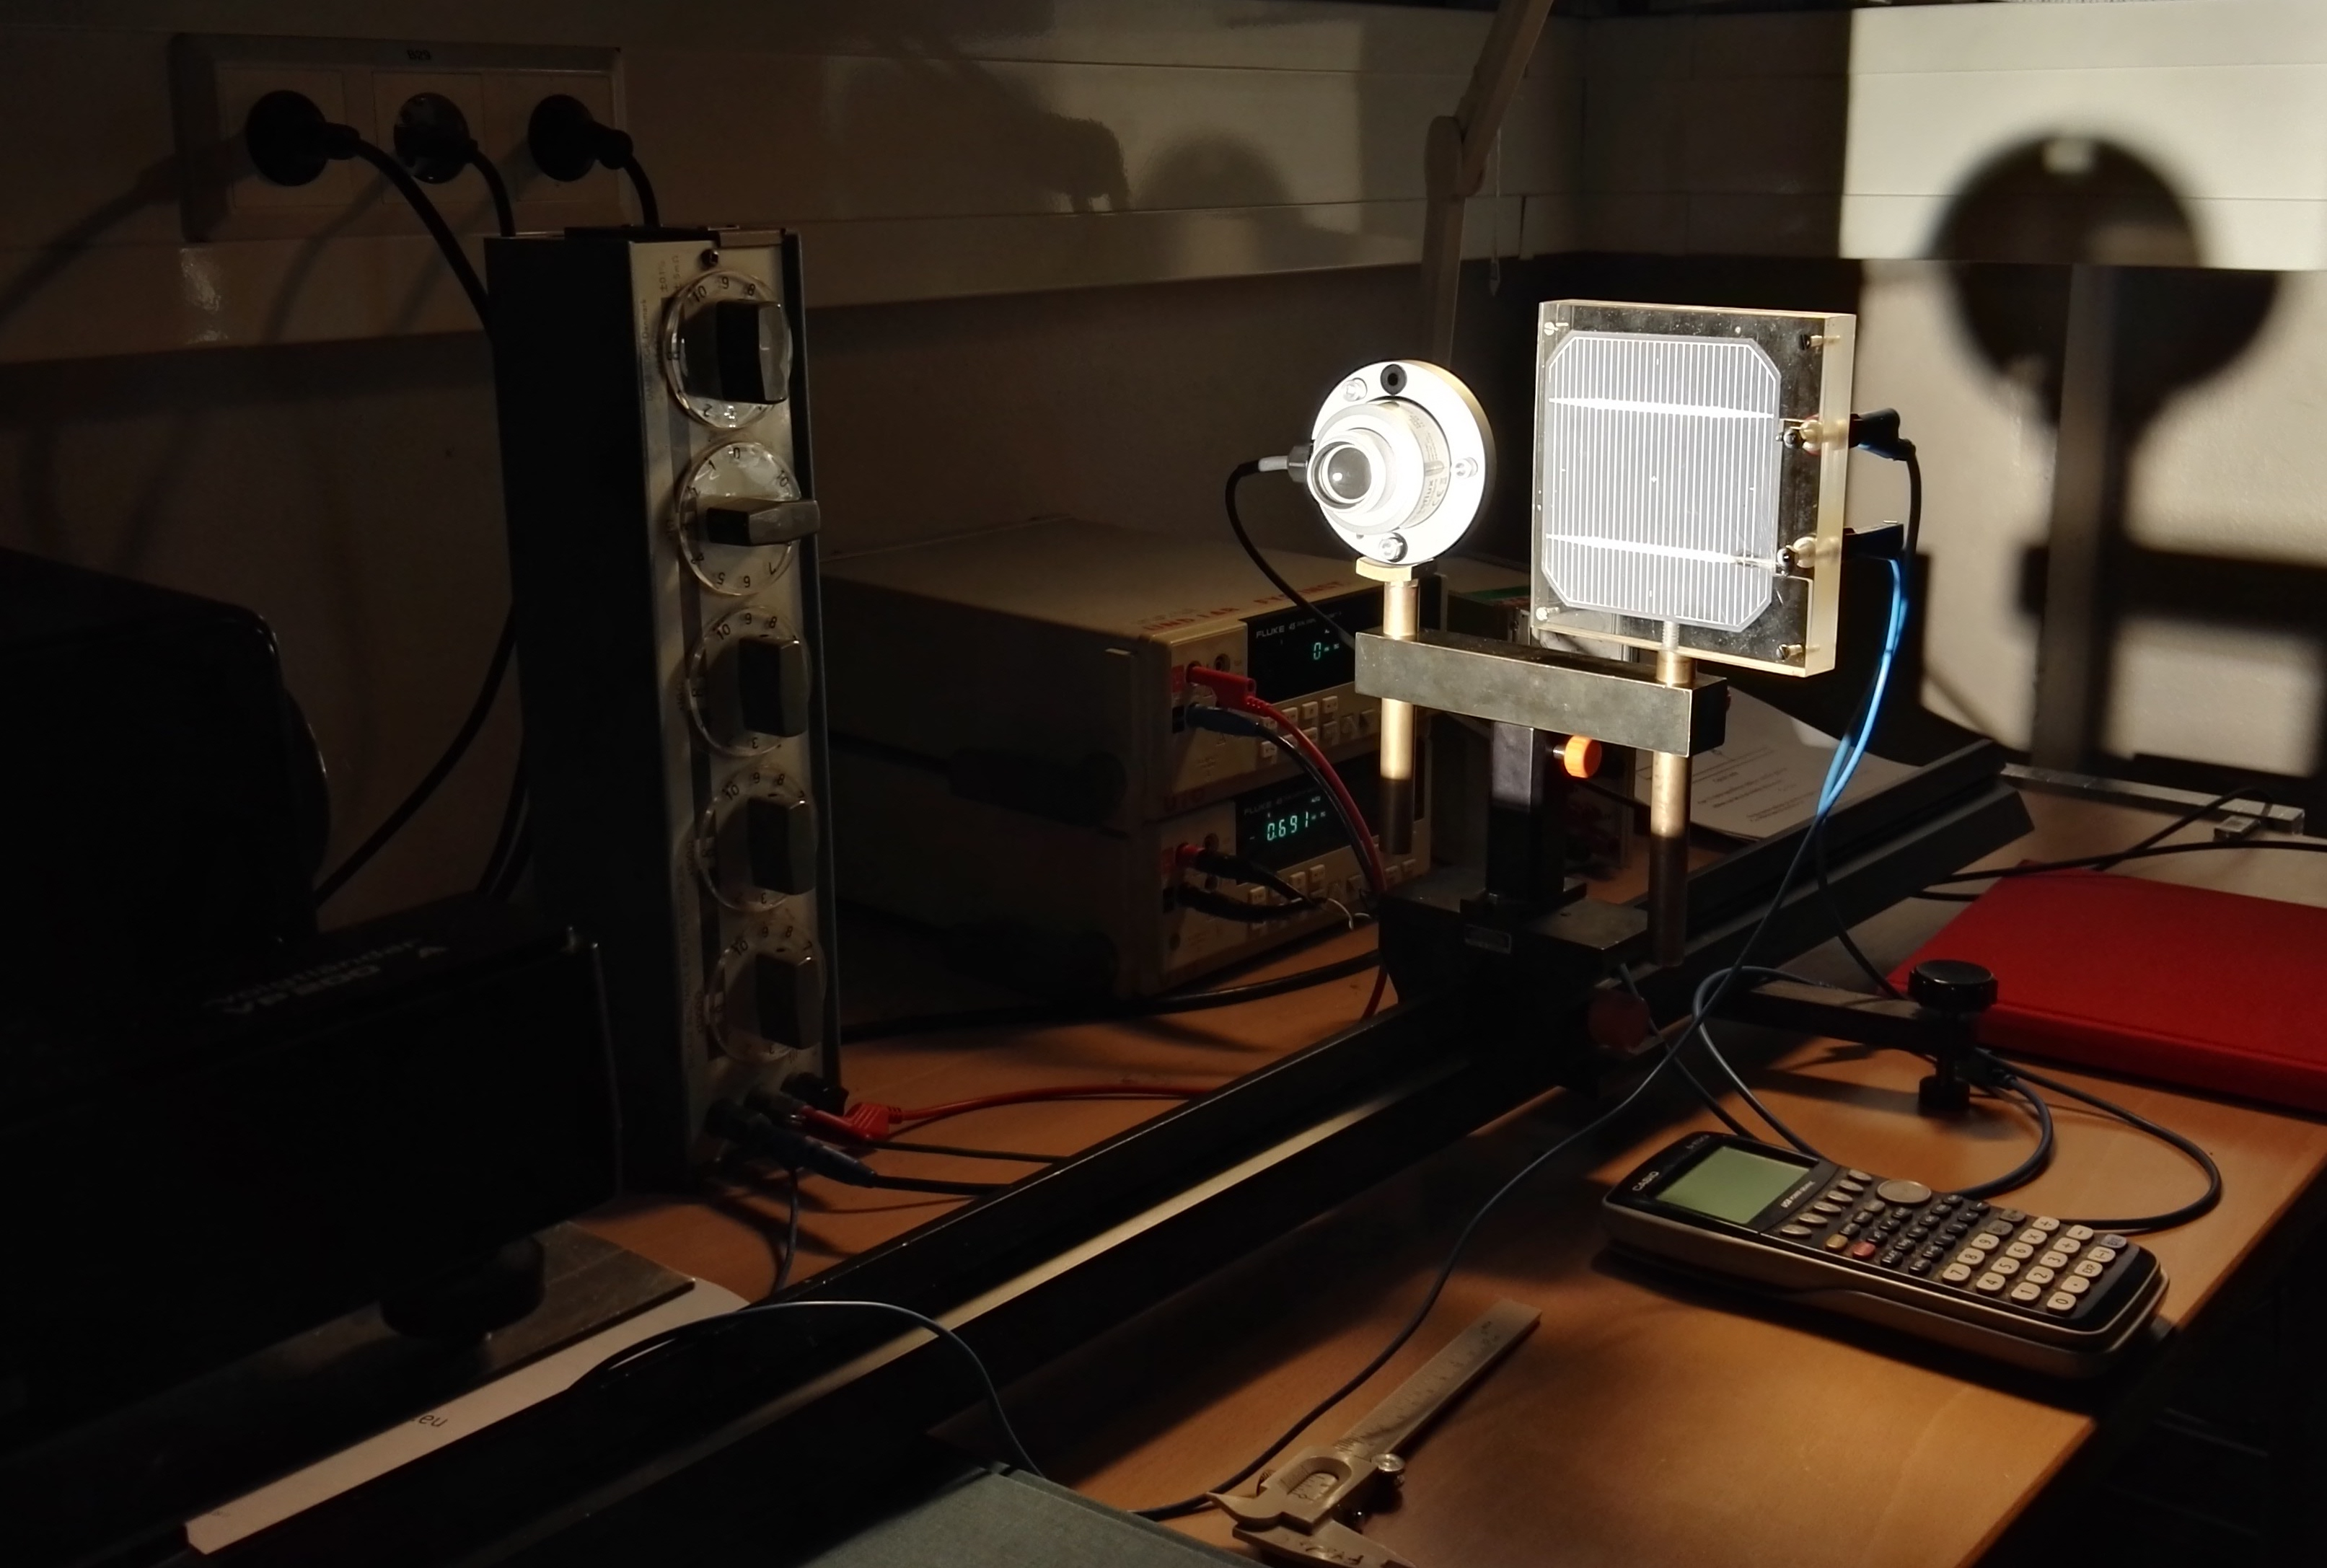
\includegraphics[scale=0.065]{lab1.jpg}
  \caption{Bilde fra laberatoriet under måling av spenningen til solarimeteret. I bildet ser vi den belyste solcellen ved siden av den belyste solarimeteret. I bakgrunnen ser vi de to multimeterene brukt under eksperimentet, og den varierende motstanden $R_L$.}
  \label{lab1}
\end{figure}
\section{Resultater}
\subsection{Strøm-spenningskarkateristikk}
For å finne strøm-spenning-spenningkarakteristikken til solcellen målte vi strømmen gjennom og spenningen over solcellen. Det ble brukt en ytre spenning på $\SI{5}{\volt}$, som ble målt til å være på $\SI{5.08\pm0.01}{\volt}$. Usikkerheten kommer fra databladet til voltmeteret. Målingene gjort strømmen og spenningen til en belyst solcelle, med en ytre spenningskilde på $\SI{5.08\pm0.01}{\volt}$, er vist i figur \vref{resultat_ytre_spenning}. I denne figuren er både målinger i positiv og negativ strømretning vist. Målepunktene viser usikkerheten i både spenning og strøm, men denne usikkerheten er for liten iforhold til endringen i strøm og spenning at den kan sees fra grafen. Kretsen brukt for generere og måle verdiene er vist i figur \vref{krets1}. \\
\begin{figure}
  \centering
  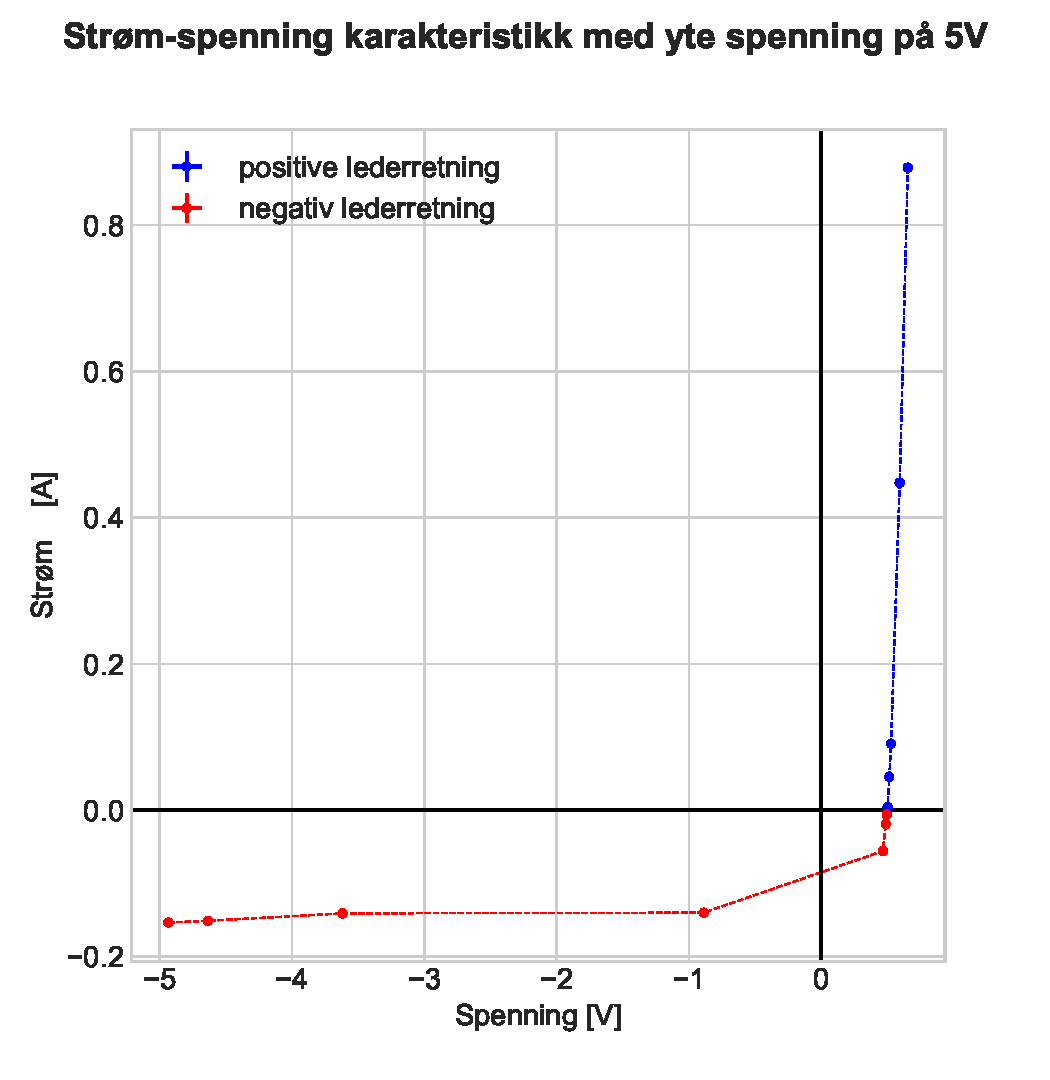
\includegraphics[scale=0.47]{ytre_spenning.pdf}
  \caption{Strøm-spenningskarkateristikken for en belyst solcelle med en ytre spenning på $5$ volt. Kretsen brukt for å gjøre disse målingene er vist i figur \vref{krets1}.}
  \label{resultat_ytre_spenning}
\end{figure}
Deretter lot vi solcellene arbeide på egenhånd ved å fjerne den ytre spenningskilden. Målinger av strøm-spenningskarkateristikken uten noen ytre spenningskilde er vist i figur \vref{resultat_uten_spenning}. Målingene for spenningen i en åpen krets, $V_{oc}$, og strømmen i en kortsluttet krets, $I_{sc}$, er markert i grafen. Verdien målt for $V_{oc}$ var $\SI{497.9\pm0.2}{\milli\volt}$, og verdien for $I_{sc}$ var $\SI{-145\pm3}{\milli\ampere}$. Usikkerheten for målepunktene i grafen stammer fra spredningen over flere målinger, og databladet til måleapparatene og motstanden brukt. \\
\begin{figure}
  \centering
  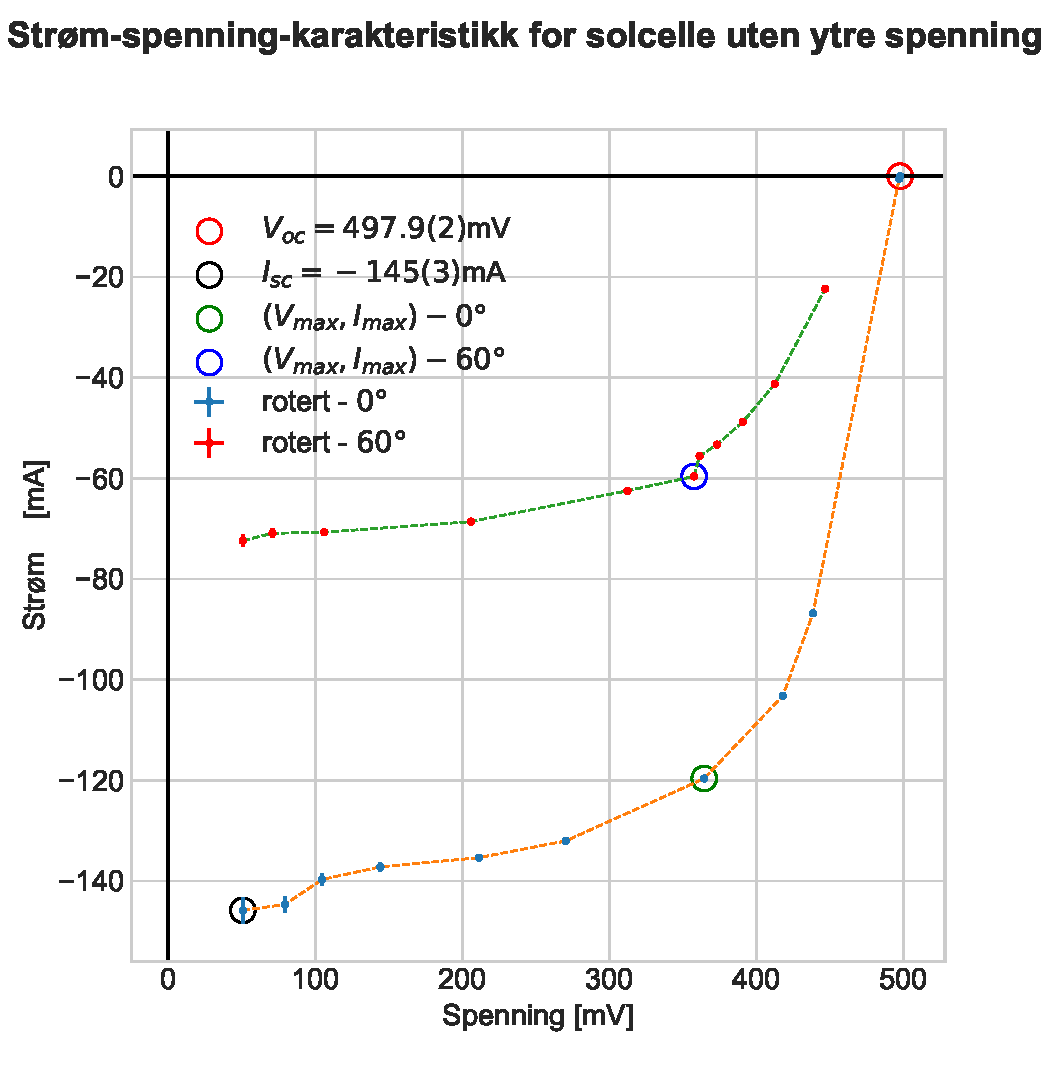
\includegraphics[scale=0.48]{strom_spenning_karr_test.pdf}
  \caption{Strøm-spenningskarkateristikken for en optimalt belyst solcelle og en delvis belyst solcelle, uten en ytre spenningskilde. Kretsen brukt for å gjøre disse målingene er vist i figur \vref{krets2}. Maksimalpunkter og $V_{oc}$ og $I_{sc}$ er markert i figuren, med verdi. Med $I_{max}$ og $V_{max}$ menes det henholdsvis ikke maksimal strøm og maksimal spenning, men henholdsvis den strømmen og den spenningen som resulterer i maksimal effekt.}
  \label{resultat_uten_spenning}
\end{figure}
For å kunne sammenlikne de to strøm-spenningskarkateristikkene er et begrenset område av verdiene vist i figur \vref{fig_ekstra}. Målingene med en ytre spenningskilde er målt i både negativ og positiv strømretning.
\begin{figure}
  \centering
  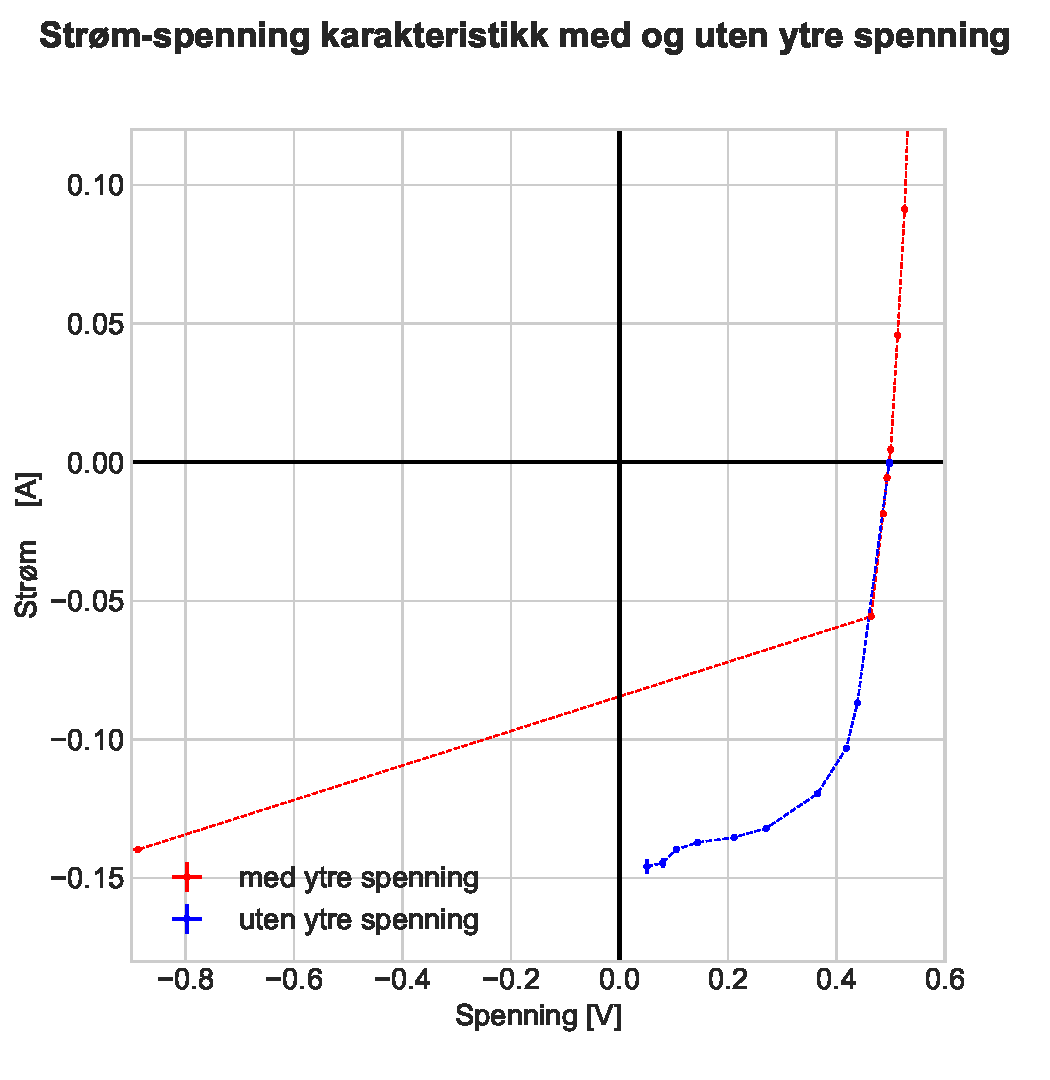
\includegraphics[scale=0.47]{ytre_spenning_sammen.pdf}
  \caption{Strøm-spenningskarkateristikken for belyst solcelle med ytre spenningskilde (figur \vref{krets1}) og uten ytre spenningskilde (figur \vref{krets2}). Den ytre spenningskilden er på $\SI{5.08\pm0.01}{\volt}$.}
  \label{fig_ekstra}
\end{figure}
\subsection{Solcellens optimale belastning}
For å finne den optimale belastningen til solcellen ble strømmen gjennom og spenningen over solcellen målt. Derfor ble målingene fra strøm-spenningskarkateristikken, vist i figur \vref{resultat_uten_spenning}, gjennbrukt, itilegg til nye målinger av en redusert belyst solcelle. Resultatet fra målingene er vist i figur \vref{maling_optimal_belast}. Den redusert belyste solcellen i figuren er dreid omlag $60\degree$ vekk fra lyskilden, dette resulterte i omtrent halvert strøm for en lav resistanse lik $\approx 0.5\Omega$.
\begin{figure}
  \centering
  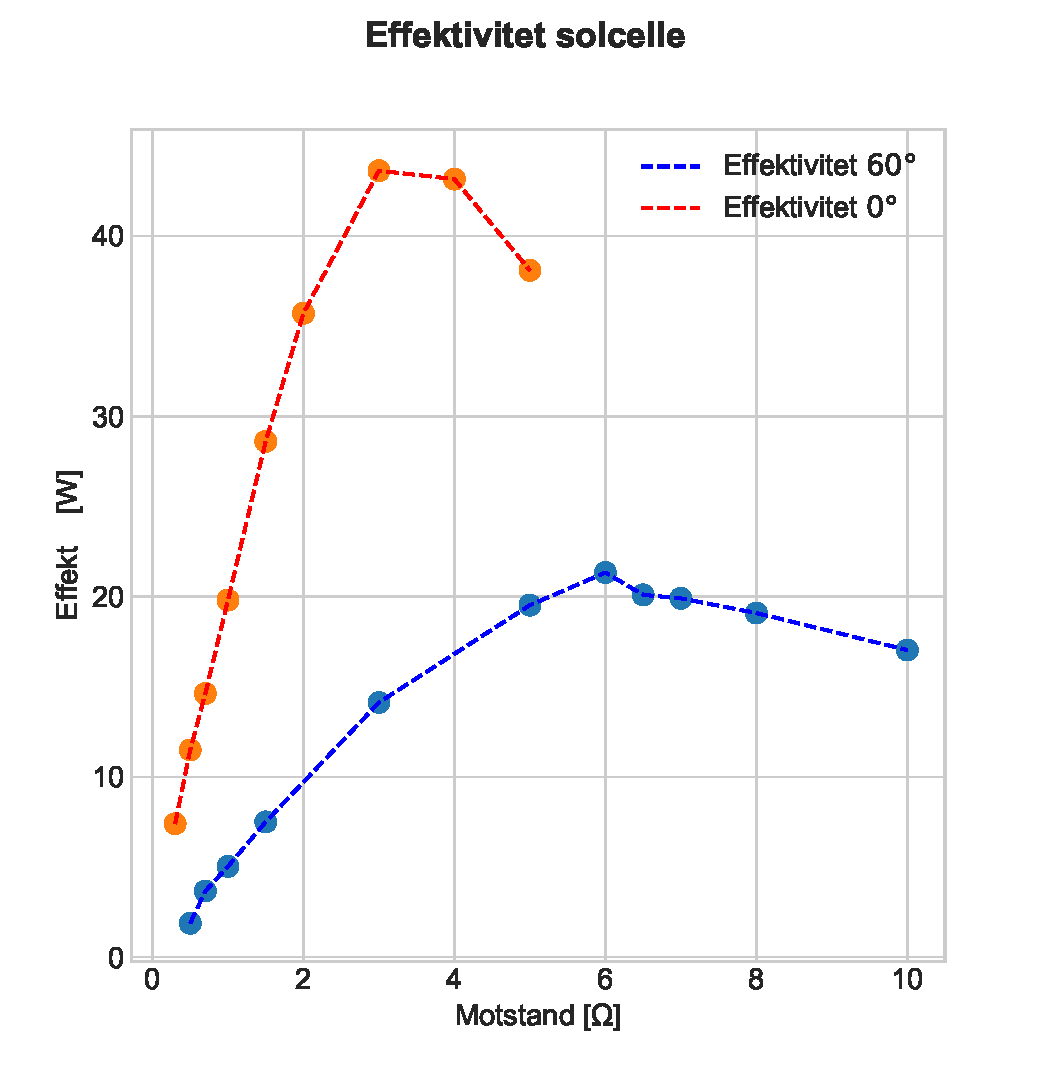
\includegraphics[scale=0.47]{effekt.pdf}
  \caption{Effekten til solcellen som en funksjon av motstanden i kretsen. Det blå datasettet er med en solcelle som er optimalt belyst, og det røde er for en solcelle som er rotert $60\degree$ vekk fra lyskilden. I figuren er de maksimale verdiene for hvert sett med måling markert og vist verdien til.}
  \label{maling_optimal_belast}
\end{figure}
Solcellen klarer å få en effekt på $\SI{43.6\pm0.1}{\milli\watt}$ når motstandslasten er på $\SI{3.00\pm0.01}{\Omega}$, strømmen i kretsen er $-\SI{119.6\pm0.3}{\milli\ampere}$ og spenningen på $\SI{364.6\pm0.3}{\milli\volt}$. For solcellen som er vendt $60\degree$ vekk fra lyskilden gir en maksimal effekt på $\SI{21.33\pm0.08}{\milli\watt}$ med en motstand på $\SI{6.00\pm0.01}{\Omega}$, en strøm på $-\SI{59.6\pm0.1}{\milli\ampere}$ og en spenning på $\SI{357.7\pm0.3}{\milli\volt}. Usikkerhetene er beregnet fra spredningen over flere målinger av samme verdi, og usikkerheten i en enkel måling fra databladet til måleappratet.
Verdien til fill factor, beskrevet ved liknign \eqref{ff}, for den fullt belyste solcellen er $0.57(1)$, og for den redsuert belyste solcellen er fill factoren lik $0.29(1)$. Støm-spenningkarakteristikken til fullt belyst og redusert belyst solcelle er vist i figur \vref{resultat_uten_spenning}.
\subsection{Kombinasjon av enkeltsolceller i et solcellepanel}
Denne målingen ble gjennomført for å måle forholdet mellom maksimal effekt for solceller under forskjellige koblinger og lysforhold. Fra å måle strømmen i en sluttet krets, og spenningen i en åpen krets, kan en finne forholdet mellom effekten i kretsen ved å bruke likning \eqref{maxP}. Det ble gjennomført målinger av de to verdiene med solcellene koblet i paralell, og serie, med begge belyst, og med en belyst. Resulatene fra målingene er vist i tabell \vref{effekt2}.
\begin{table}[h]
\renewcommand\arraystretch{1.3}
\begin{adjustwidth}{-0.3in}{0.1in}
\begin{tabular}{|l | *{3}{>{\centering}p{2cm}|}c|}
\hline Kobling & \multicolumn{2}{c|}{Parallell} & \multicolumn{2}{c|}{Serie} \\
\hline Måling & $V_{oc}$[mV]    &   $I_{sc}$ [mA]  &   $V_{oc}$ [mV]  &  \,\,\,\,\,\,$I_{sc}$ [mA]\,\,\,\,\,\, \\
\hline Begge belyst & 499.8(3)    &   -293(3)  &   1000.9(9)  &  -139(2)\\
\hline En belyst    & 461.53(2)    &   -155(2)  &   634.7(3)  &  -0.428(5)\\ \hline
\end{tabular}
\end{adjustwidth}
\caption{Målinger gjort av spenningen i en åpen krets, og strømmen i en kortsluttet krets. Fra disse verdiene kan det beregnes forholdet mellom effektiviteten til de forskjellige tilfellene.}
\label{effekt2}
\end{table}
Fra å bruke likning \eqref{maxP} på dataen vist i tabell \vref{effekt2} kan en beregne fram til informasjon om de relative effektene for forskjellige koblinger og lysforhold. Når vi har begge solcellene belyst er effekten omtrent lik. Parallellkoblede solceller gir en faktor $1.05(2)$ mer effekt iforhold til at solcellene koblet i serie når begge solcellene er belyst. Derimot hvis bare en av solcellene er belyst er det en faktor $263(3)$ mer effekt fra å ha solcellene i parallell iforhold til å ha solcellene i seriekobling. For solceller koblet i parallell viser det seg at effekten når begge er belyst er en faktor $2.04(1)$ større enn når én solcelle er belyst i parallellkobling. For solceller koblet i serie er det en faktor $512(7)$ mer effekt å ha begge solcellene belyst, istedenfor bare en av de to solcellene belyst. Usikkerhetene er beregnet fra spredningen over flere målinger og usikkerheten i en enkelt måling fra måleinstrumentet. Disse usikkerhetene er brukt videre for å beregne usikkerheten i forholdet mellom effekten under de forskjellige forholdene. Usikkerheten i å anta at fill-factor konstant er ikke tatt med i betraktning. Fra å bruke verdien beregnet for fill factor, kan vi bruke likning \eqref{ff} til å finne den maksimale effekten fra å ha to koblede solceller. Beregninene gir oss at den maksimale effekten er $\SI{83\pm1}{\milli\watt}$.
\subsection{Solcellens virkningsgrad}
Ved å plasere et solarimeter ved samme avstand til lyskilden som solcellen kan en beregne effektiviteten til solcellen. Solarimeteret som ble brukt under eksperimentet hadde kalibreringskonstant $a=\SI{11.13}{\micro\volt\meter^2\per\watt}$. Ved å bruke et skyvelær for å måle de forskjellige geometriske størrelsene til solcellen, kan en beregne at arealet til solcellen er $\SI{96.3\pm0.2}{\centi\meter^2}$. Usikkerheten kommer fra databladet til skyvelæret brukt under målingene. Gjennomsnittet av flere målinger til spenningen over solarimeteret viste seg å være $\SI{686.2\pm0.3}{\milli\volt}$, hvor usikkerheten kommer fra spredningen over flere målinger, og usikkerheten i en måling fra databladet til voltmeteret. Fra disse verdiene kan en bruke likning \eqref{kalibrering} til å vise at den innstråle effekten er
$\SI{593\pm(2)}{\milli\watt}$. Denne verdien, sammen med den maksimale effekten som har blitt målt fra solcellen, vist i figur \vref{maling_optimal_belast}, til å være $\SI{43.6\pm0.1}{\milli\watt}$, kan vi beregne virkningsgraden til solcellen med likning \eqref{effekt}. Vi finner at effekten til solcellen er $7.35(3)\%$. Hadde solcellen i dette eksperimentet hatt et areal på $\SI{1}{\meter^2}$ ville den nådd en effekt på $\SI{4.52\pm0.01}{\watt}$.
\section{Diskusjon}
\subsection{Strøm-spenningkarakteristikk}
Målingen av strøm-spenningkarakteristikk ble gjort med og uten en ytre spenningskilde. Fra å se på målingene med en ytre spenningskilde, vist i figur \vref{resultat_ytre_spenning}, kan en se en viktig egenskap med solceller. Solceller leder strøm i en retning, men ikke i en annen. Solcellen oppfører seg som en diode. Årsaken til dette er at når man snur polariteten til spenningen vil en bare kontaktpotensialet på $pn$-overgangen øke, og dette gjør at det ikke vil kunne lede noe strøm over solcellen. Når strømmen går i positiv lederretningen har vi et positivt spenningsfall over solcellen, og positiv strøm i kretsen. Forholdet mellom strømmen og spenningsfallet ser ut til å øke eksponesielt. Ved å snu polariteten på spenningskilden ble det gjort målinger av strøm-spenningkarakteristikk i negativ lederrtening. Disse målepunktene sier oss at strømmen i kretsen går mot en lav og konstant verdi, når spenningen går mot null og blir negativ, når strømmen beveger seg i sperreretning. Når motstanden er minst skjer all spenningsfallet over solcellen, for høyere motstander nærmer strømmen i kretsen seg $0$, men går aldri over på grunn av polariteten på spenningskilden. På grunn av at forholdet mellom strøm gjennom og spenning over solcellene er en krom linje, viser dataene at en solcelle er en ikke-lineær komponent. Målepunktene som er i første og tredje kvadrant er strøm-spenning-forhold der solcellen konsumerer effekt, men for målepunkter i fjerde kvadrant generer solcellen effekt. Altså er det kunn noen kombinasjoner av strøm og spenning, hvor alle er i negativ lederretning, hvor solcellen generer effekt, når det er en ytre spenningskilde \cite{torbj}. \\Siden solcellen er en diode burde det ikke gå noe strøm i kretsen når polariteten til spenningskilden er snudd, men målingene viser at det går en strøm. Denne strømmen kalles lekasjestrøm, som oppstår fra $pn$-overgangen i en diode når polariteten er snudd. Forflytningen av ladninger skyldes spenningen over $pn$-overgangen som gjør at elektroner fra $p$-siden blir dratt mot spenningskildens positive side, og hullene på $n$-siden blir dratt mot spenningskildens negative side. \par
Målingene gjort av strøm-spenningskarkateristikken uten en ytre spenningskilde er vist i figur \vref{resultat_uten_spenning}. La oss første se på målingene for den fullstendig belyste solcellen. Kurven på grafen er slik en forventer for en belyst solcelle. For lave resistanser flater strømmen ut mot en konstant verdi, som går mot $I_{sc}$. For høyere motstander øker strømmen eksponensielt, og skjærer $x$-aksen i $V_{oc}$ hvor kretsen er åpen, det vil si uendlig motstand. Den maksimale spenningen fra en enkelt solcelle går mot $\SI{0.5}{\volt}$. For å bestemme $I_{sc}$ kunne det ikke brukes en kortsluttet, hvis resistansen til motstanden er null, vil også spenningen vi måler vise null, dette gjør at det blir umulig å måle en verdi for $I_{sc}$. Under målingene ble det derfor brukt en motstand på $\SI{0.5}{\Omega}$, grunnen til at det ikke ble valgt en lavere motstand er at for en så lav resistanse vil lednings- og kontakt-resistanser ha en effekt på spenningsfallet i kretsen, og er noe som vi ikke klarer å måle under eksperimentet. Siden kurven flater ut når spenningen minker blir den svakeste motstanden som gir et konstant spenningsfall over motstanden brukt for å måle $I_{sc}$. Som en ser i grafen virker dette som en god tilnærming av $I_sc$. Av å bestemme den maksimale effekten til solcellen finner en det største arealet mulig innenfor kurven i den fjerde kvadrant. Målingene av spenningen gjør et lite rykk ned for de to laveste målepunktene. Årsaken til dette kan være noe systematisk feil under eksperimentet sp, istabiliteter i lysstyrken eller ikke-ideelle koblinger. Det burde merkes at for disse målepunktene er usikkerheten i strømmen større enn for de andre målepunktene. Fra at linjen gjennom målepunktene er krom kan det sluttes at solceller er ikke-lineære komponenter. Siden alle datapunktene er i fjerde kvadrant betyr dette at solcellen generer effekt i kretsen. \\
For den svakere belyste solcellen som er rotert $60\degree$ vekk fra lyskilden er formen på kurven den samme, men med en lavere strøm. Det ser ut til at spenningen over solcellen er det samme for begge belysninger. En ser også at det er for omtrent samme spenning at de to kurvene oppnår maksimal effekt. Det kunne vært spennende å gjøre flere målinger av dette, med forskjellig belysninger for å se om $V_{max}$ varierer eller ikke. Fra grafen ser man at det vil bli generert mindre effekt for den mindre belyste solcellen. Under eksperimentet burde det blitt målt $V_{oc}$ for den mindre belyste solcellen, fra figuren kan det virke som at begge kurvene går mot samme verdi for $V_{oc}$, men på grunn av mangel på måleresultater kan vi ikke trekke denne slutningen, men er noe som burde sees nøyere på i et senere eksperiment.\par
De to strøm-spenningkarakteristikkene er vist sammen i figur \vref{fig_ekstra}. Fra målepunktene er det lett å se at de to kurvene passer godt sammen. Desverre ble det ikke gjort flere målinger av strøm-spenningkarakteristikken i negativ strømretning. Men fra å vite at strømmen også skal flate seg ut når spenningen går mot null, og at de to kurvene flater ut mot samme verdi, er det fristende å slutte at de to kurvene ville fortsatt å følge hverandre. En forklaring på at de  to grafene ser ut til å beskrive det samme kan være at når vi måler $I_{sc}$ vil det ikke være noe spenningsfall over solcellen, og for dette tilfellet vil det bare være lekasjestrøm som går i kretsen, og de to verdiene burde derfor gå mot samme verdi. \\
Årsaken til at det ble brukt et voltmeter og en motstand for å beregne strømmen gjennom kretsen istedenfor et amperemeter, er at når solcellen er den eneste speningsforskyneren til kretsen kan den indre motstanden i et amperemeter være for stor, slik at solcellen ikke kan yte maksimalt. Dekademotstanden brukt som erstatning hadde en stor usikkerhet i motstanden, iforhold til usikkerheten målt i spenningen, fra spredning og datablad, som gjør at det er en mye større usikkerhet i strømmen enn i spenningen. Dette kan en se tydelig i figur \vref{resultat_uten_spenning}. Denne effekten er hovedsaklig merkbar for lave motstander, grunnet det høye konstantleddet i usikkerheten i dekademotstanden.
\subsection{Solcellens optimale belastning}
Fra å se på grafen over effekten til solcellen, vist i figur \vref{maling_optimal_belast}, er det to ting å merke seg. Den første, og den mest selvfølgelig, er at solcellen som blir sterkere belyst gir en større effekt. Den andre er at hvilken lastmotstand som resulterer i maksimal effekt avhenger av bestrålingen. For den fullt belyste solcellen er resistansen som resulterer i størst effekt $\SI{3.00(1)}{\Omega}$, for den redusert belyste er resistansen $\SI{6.00(1)}{\Omega}$. Dette er en viktig egenskap ved solceller i krets. Ønsker man en størst mulig effekt fra solcellen burde lasten i kretsen variere med belysningen av solcellen. Fill factoren beregnet for den fult belyste solcellen er $0.57(1)$, og sier oss hvor mye effekt vi får ut fra solcellen vår. For vanlige solceller er det vanlig at fill factor er på rundt $0.7-0.8$ for optimalt belyste solceller \cite{energy_alt}. Som vi har sett har solcellen brukt i dette eksperimentet en lavere effekt, og derfor en lavere fill factor. For den redusert belyste solcellen er fill factoren enda lavere, $0.29(1)$, siden det er en mindre belysning, og derfor enda mindre effekt iforhold til den optimale verdien av fill factor, som er $1$. I eksperimentet ble det ikke målt $V_{oc}$ for den redusert belyste solcellen, dette burde ha blitt gjort for å kunne sammenlikne fill factoren for de to belysningene, istedenfor å bruke samme verdi for $I_{sc}$ og $V_{oc}$ i begge beregningene.
\\Den maksimale effektforskjellen, og den optimale belastningen og den optimale strømmen, er ganske lik en faktor to forskjellig mellom den fullt og redusert belyste solcelle. Om dette forholdet fortsetter å være proposjonalt er noe som det ikke var tid til å måle under dette eksperimentet, men denne sammenhengen er noe som burde måles i et annet eksperiment for å se nærmere på sammenhengen.\\ I figur \vref{maling_optimal_belast} har de to største verdiene for effekten, for den fullt belyste solcellen, nesten samme verdi. Dette kan bety at den optimale belastningen ligger i området mellom disse to målepunktene, det vil si mellom $6\Omega$ og $6.5\Omega$. En konsekvensen av dette ville være at den maksimale effekten funnet for solcellen er litt lavere enn den faktisk maksimale effekten. Dette har isåfall påvirket virkningsgraden til solcellen, og kan ha vært med på å føre til at den er lavere enn å forvente.
\subsection{Kombinasjon av enkeltsolceller i et solcellepanel}
Fra målingen vist i tabell \vref{effekt2} er det lett å se at det å koble flere solceller i serie øker spenningen i kretsen, og koble solceller i parallell øker strømmen. Begge disse egenskapen vil dobbles iforhold til den den andre koblingen. Fra tabellen kan en også se effekten av å bestråle to solceller iforhold til en, og hvordan koblingsmåte påvirker dette. For parallellkobling halveres strømmen, men spenningen er nesten uforandret, når det blir belyst en solcelle istedenfor to. For seriekobling synker både strøm og spenning. Spenningen blir litt under halvert, men strømmen blir redusert med en faktor på over $300$. \par
Ved å bruke likning \eqref{maxP} kan en beregne forholdet mellom effekten for de forskjellige tilfellene. Det er da viktig å huske på at denne likningen er en tilnærming. Fill factor antas å være en karakteristikk ved solcellen som ikke er avhengig av ytre forhold. Dette gjør at den er tilnærmet konstant, og denne tilnærmingen skaper en usikkerhet i forholdet mellom effektene. Denne tilnærmingen er ikke tatt med i usikkerheten til effekten. Denne usikkerheten er kunne beregnet fra spredningen til en serie av målinger til $I_{sc}$ og $V_{sc}$ og databladet til måleapparatene. For å få en mer nøyaktig, og spesifikk verdi for effekten, kunne strøm-spenningkarakteristikken for solcellene blitt målt individuelt under alle forholdene. Dette ble ikke gjort under eksperimentet grunnet tidsbegrensninger. Fra å se på forholdet mellom effektene for de ulike koblingene og lysforholdene kan en gjøre flere slutninger om hvordan en kan få mest ut av solceller. Når bare en solcelle er belyst gir det en faktor $263(3)$ mer effekt å ha solcellene koblet i serie i forhold til parallell. Årsaken til dette er at solceller oppfører seg som en diode når de ubelyst, det vil ikke føre strøm. Derfor vil kretsen kortsluttes når kunn den ene solcellen er belyst. For en parallellkobling vil dette ikke føre til at kretsen blir kortsluttet, siden den belyste solcellens påvirkning i kretsen ikke vil bli merket av den andre solcellen. Derimot for seriekoblede solceller vil en ubelyst solcelle ødlegge strømførselen i kretsen, og reduserer effekten dramatisk. Akkurat som målingene viser. Fra disse målingene ser en at det er ekstremt viktig at alle solcellene er belyst når de kobles i serie. Målingene viste at vi fikk omtrent samme effekt for å ha begge solcellene belyst under serie og parallell. Parallellkobling gir en litt større effekt som er en faktor $1.05(2)$ større enn effekten fra seriekoblingen. Vi fant også at effekten fra to solceller var $\SI{83\pm1}{\milli\volt}$, som er en faktor $1.90(2)$ mer enn den maksimale effekten fra en enkel solcelle.
\\
Etter å ha gjort målingene med de to solcellene målte vi virkningen på spenningsfallet over resistansen av å bytte posisjonen til de to solcellene. Målingen viste en spenningsforskjell på $\SI{3}{\milli\volt}$. Denne forskjellen har derfor blitt tatt med i usikkerhetsberegningene for de relative effektene.
\subsection{Solcellens virkningsgrad}
Under beregning av arealet tok vi hensyn til formen på solcellen, som en ser i figur \vref{lab1}, men det ble ikke tatt hensyn til fingrene på tverrs av solcellen. Dette kan ha påvirket den endelige effekten, men utslaget til effekten av solcellen av å inkludere dette ville vært minimalt.\\
Målingen av den maksimale effekten, og målingen av solarimeteret ble gjennomført med over en time mellomrom. Iløpet av denne tiden er det mulig det har vært noen uønskede forandringer på eksperimentet som kan ha forårsaket systematiske feil, for eksempel forandring av belysning i rommet, forandring av solcellens avstand til lyskilden eller intensiteten til lyskilden. Solcellen forventet å ha en effektivitet på rundt $10\%$, og det kan ha vært systematiske feil som disse som forårsaket avviket. Det er også mulig at solcellen ble plassert for langt vekk fra lyskilden under eksperimentet, og at denne avstandsforskjellen redusert intensiteten, som førte til en lavere strøm i kretsen, og en lavere effekt fra motstanden.\\
Årsaken til at en forventer en så lav virkningsgrad som $10\%$ i dette eksperimentet, når komersielle solceller er på rundt $15$ til $22\%$, er at i vårt eksperiment blir det ikke brukt sollys som belysning. I vårt eksperiment er den eneste lyskilden en lysprojektor, som ikke vil gi samme spredning av forskjellige bølgelengder som lys fra sola. Lys fra sola inkluderer korte bølgelengder utenfor det synlig spekteret som bærer mye energi. Det er viktig å ha fotoner med høy nok energi for å kunne løsrive elektronene og danne elektron-hull-par. Denne delen av spekteret er muligens ikke like godt dekket av lysprojektoren, siden den har ikke som hensikt å produsere fotoner utenfor det synlige spekteret. Dette kan være en av årsakene til at solcellen gir en lavere virkningsgrad enn det som forventes av solceller.
\section{Konklusjon}
I dette eksperimentet har det blitt gjort flere målinger på solceller i forskjellige koblinger og lysforhold. Fra å analysere disse målingene har det blitt gjort flere slutninger om hvordan å maksimere effekten fra solceller.\\
Fra å se på strøm-spenning karakteristikken til en solcelle,
med (figur \vref{resultat_ytre_spenning}) og uten (figur \vref{resultat_ytre_spenning}) en ytre spenningskilde, kan vi se at en solcelle oppfører seg som en diode, i den fortstand at den bare leder strøm i en retning. \\
De samme målingene kan brukes til å beregne den maksimale effektiviteten til en solcelle. Dette ble gjort for en total belyst solcelle, og en devil belyst solcelle. Denne målingen er vist i figur \vref{maling_optimal_belast}, og forteller oss at den optimale motstandsbelastningen er en funksjon av belysningen av solcellen. Dette er en viktig egenskap ved solceller, som må utnyttes for å kunne få mest mulig effekt fra et solcellepanel.\\
I eksperimentet ble det gjort målinger av hvordan forskjellige lysforhold påvirket effekten for forskjellige koblingsmåter. Disse målingene er vist i tabell \vref{effekt2}, og gir oss mye informasjon om hvordan å maksimere solceller. For å øke strømmen burde solceller kobles i parallell, men ønsker man økt spenning burde de kobles i serie. Det forteller oss også at det er viktig at begge solcellene er belyst når de er koblet i serie. Årsaken til dette er at en ubelyst solcelle vil stoppe strømmen i kretsen, dette fører til en faktor $512(7)$ mindre effekt i kretsen. For parallellkoblinger blir effekten redusert med en faktor $0.49(1)$, grunnet at bare den ene solcellen i kretsen vil være til nytte. Hvis bare en av solcellene skal være belyst er det en faktor $263(3)$ mer effekt av å solcellene koblet i serie.\\
Ved å bruke et solarimeter kunne forholdet mellom den bestrålte effekten og den genererte effekten fra solcellen beregnes. Det ble målt at virkningsgraden til solcellen var $7.35(3)\%$. Årsaken til den lave verdien er at lyskilden var en projektor, og ikke solen, som sender elektromagnetisk stråle over en større del av det elektromagnetiske spekteret.
\subsubsection*{Utstyrsliste}
\begin{itemize}
\label{utstyr}
\item meterstokk - Hultafors
\item Lysprosjektor - Voigtländer
\item Voltmeter (2) - Fluke 45
\item Dekademotstand - Danbridge DR5/ABCDE
\item Optisk benk
\item Spenningskilde
\item Solcelle (2)
\item Solarimeter
\item Ledninger
\end{itemize}
\begin{thebibliography}{9}
\bibitem{squires}
Squires, G.L. \emph{Practical Physics}, Cambridge University Press, 2001.
\bibitem{oppgave}
Fysisk institutt, \emph{FYS 2150. SOLCELLEN}, Univseritet i Oslo, februar 2017.
\bibitem{torbj}
Robert T. Paynter, B.J. Toby Boydell, \emph{Electronics Technology Fundamentals}, Pearson second edition, 2005.
\bibitem{snl}
Lars Mæhlum, \emph{solceller}, \url{https://snl.no/solceller}, Store norske leksikon, sist oppdatert 30. oktober 2017, hentet 24. april 2018.
\bibitem{snl2}
Knut A. Rosvold, Knut Hofstad \emph{solenergi}, \url{https://snl.no/solenergi}, Stor norske leksikon, sist oppdatert 17. desember 2017, hentet 24. april 2018.
\bibitem{energy_alt}
Karl Ochsner \emph{Solar Cell I-V Characteristic} \url{http://www.alternative-energy-tutorials.com/energy-articles/solar-cell-i-v-characteristic.html} Alternative Energy Tutorials, sist oppdatert april 2018, hentet 25. april 2018.
\end{thebibliography}
\end{document}
